%!TEX root = bachelor.tex
\chapter{Methodik}
\label{ch:method}

In diesem Kapitel stellen wir ein Verfahren vor, dass ermöglicht anhand eines Bildes (siehe Einleitung).

Zunächst gehen wir auf das verwendete Kalibrierungsmuster ein, woraufhin die genaue Vorgehensweise zur Entfaltung erläutert wird. 

Die geometrischen Eigenschaften des Kegelstumpfs $(r, R, \Delta H)$ können gemessen und somit als bekannt angenommen werden. 
Darüber hinaus nehmen wir an, dass sich das Zentrum des kleineren Kreises im links-händigen Weltkoordinatensystem an der Positon $(0,0,0)$ (siehe Abbildung \ref{fig:coneFrustum}) befindet. Durch diese Einschränkung gehen jegliche absolute Größenverhältnisse verloren. Es ist also nicht mehr möglich die Größe einer Larve zu bestimmen. 

Wir wollen eine Beziehung zwischen Bildpunkte und Kegelpunkten herstellen. wo ist z achse?


\section{Kalibrierungsmuster}
\label{s:calibrationPattern}
Um eine Beziehung zwischen Bildpunkten und Kegelpunkten herstellen zu können, ist ein Kalibrierungsmuster notwendig.

Die Wahl des Kalibrierungsmusters spielt dabei eine entscheidende Rolle bei der Robustheit und Präzision der Entfaltung. Es muss gewährleistet sein, dass die charakteristischen Merkmale des Musters, auch bei leichten Abweichungen der Kamera vom Lot und schlechteren Beleuchtungssituationen zuverlässig erkannt werden. Das Muster muss darüber hinaus so entworfen sein, dass beim zusammenlegen im Kegel, dessen geometrische Eigenschaften nicht verfälscht, sondern realitätsgetreu wiedergeben werden. 

Wir haben uns für ein Muster entscheiden, dass in äquidistanten Abständen $\Delta R$, beginnend mit dem kleinen Radius $r$ des Kegelstumpfs (siehe Abbildung \ref{fig:coneFrustum}) Kreislinien und in gleichen Winkelabständen $\Delta \alpha$ auf der Seitenhöhe Liniensegmente besitzt. Das zusammengelegte Muster ist in Abbildung \ref{fig:calibrationPatternTop} zu sehen, beziehungsweise das entfaltete in \ref{fig:calibrationPattern}. Die Anzahl der Kreislinien wird mit $n$ gekennzeichnet, die Anzahl sichtbarer Liniensegmente im Kegel mit $m$. Zu beachten ist, dass bedingt durch das Entfalten, in \ref{fig:calibrationPattern}  ein Liniensegment doppelt zu sehen ist. Die schwarzen Kreise bezeichnen wir als Samples. 

Dadurch dass die Geometrie des Kegels bekannt ist, kann jedem Sample nun ein Punkt auf dem Kegel im Weltkoordinatensystem zugeordnet werden. Da ein Kegel beliebig um die $Y$ Achse rotiert werden, kann ist diese Abbildung zunächst nicht eindeutig. Dazu nehmen wir an, dass das Liniensegment mit dem kleinsten Winkel zur $X$-Achse mit dem Kegelwinkel $\theta = 0$ korrespondiert (siehe \ref{eq:paramFrustum}).

\begin{figure}[!htb]
	\centering
	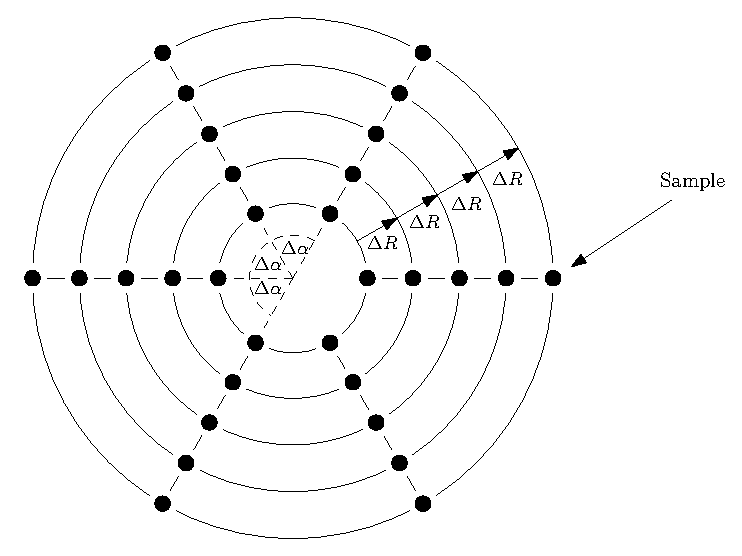
\includegraphics[scale=.8]{images/calibrationPatternTop.eps}
	\caption{Kalibrierungsmuster von oben mit $n = 5, m = 6$}
	\label{fig:calibrationPatternTop}
\end{figure}


\begin{figure}[!htb]
	\centering
	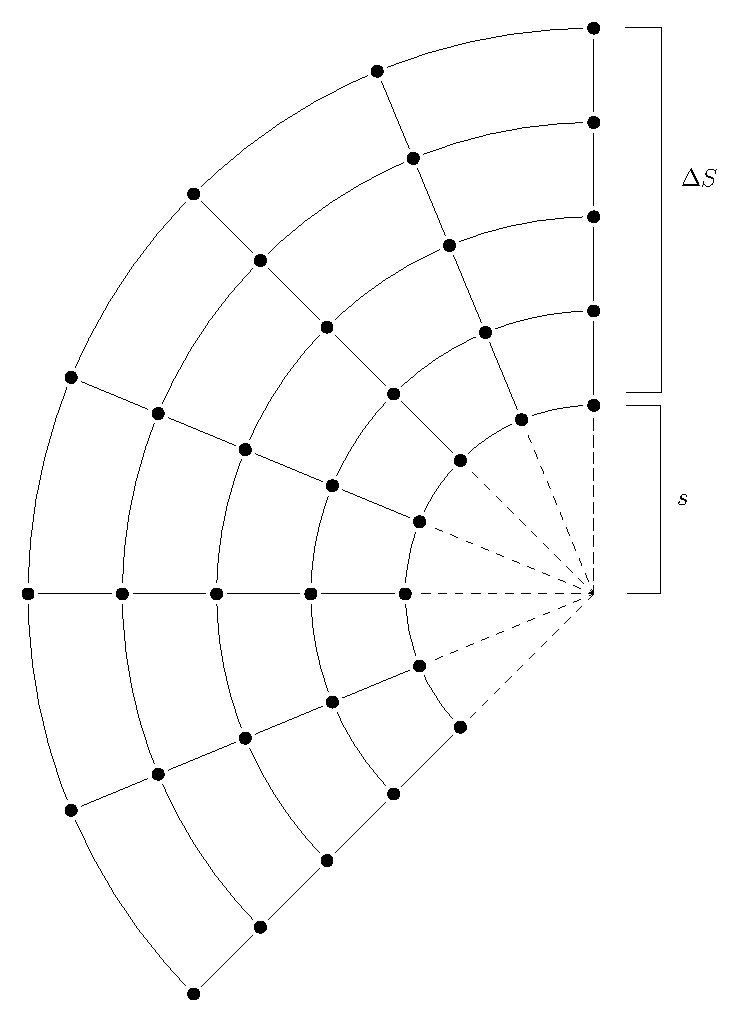
\includegraphics[scale=.7]{images/calibrationPattern2.eps}
	\caption{Kalibrierungsmuster entfaltet mit $n = 5, m = 6$}
	\label{fig:calibrationPattern}
\end{figure}

Das Muster ist also 

\subsection{Anzahl der Samples}
Die Anzahl der Samples sollte groß genug sein, um möglichst viel geometrische Informationen des Kegels zu erhalten, aber klein genug, dass eine Detektion der Samples problemlos möglich ist. Insbesondere auf dem innersten Kreis, macht sich eine zu hohe Sampleanzahl negativ bemerkbar, da der Abstand zueinander sehr klein wird, was eine Detektion erschwert. Des Weiteren sollte noch ein möglichst großer Teil der Kreislinie zu sehen bleiben, da diese für die Ellipsendetektion benötigt werden. \todo{siehe später, dazu mehr später????}


\todo{warum gerade dieses muster? warum ist das so gut? wie berechnet man das muster? welche eigenschaften hat es?}


Bilder von kegel mit muster drin?

\section{Intrinsische Kamerakalibrierung}

Bedingt durch die Wahl einer Weitwinkelkamera, enthält die Linse der Kamera eine starke tonnenförmige (nach außen gewölbte) Verzerrung. Ohne eine intrinsische Kamerakalibrierung würde. Es werden nur die intrinsischen Parameter benötigt. \todo{ Warum die extrinsciehn nicht? kamera postion gegeben dann ??}

\todo{Vergleich ohne und mit Kalibrierung}

\begin{figure}[!htb]
	\centering
\begin{subfigure}{.5\textwidth}
	\centering
	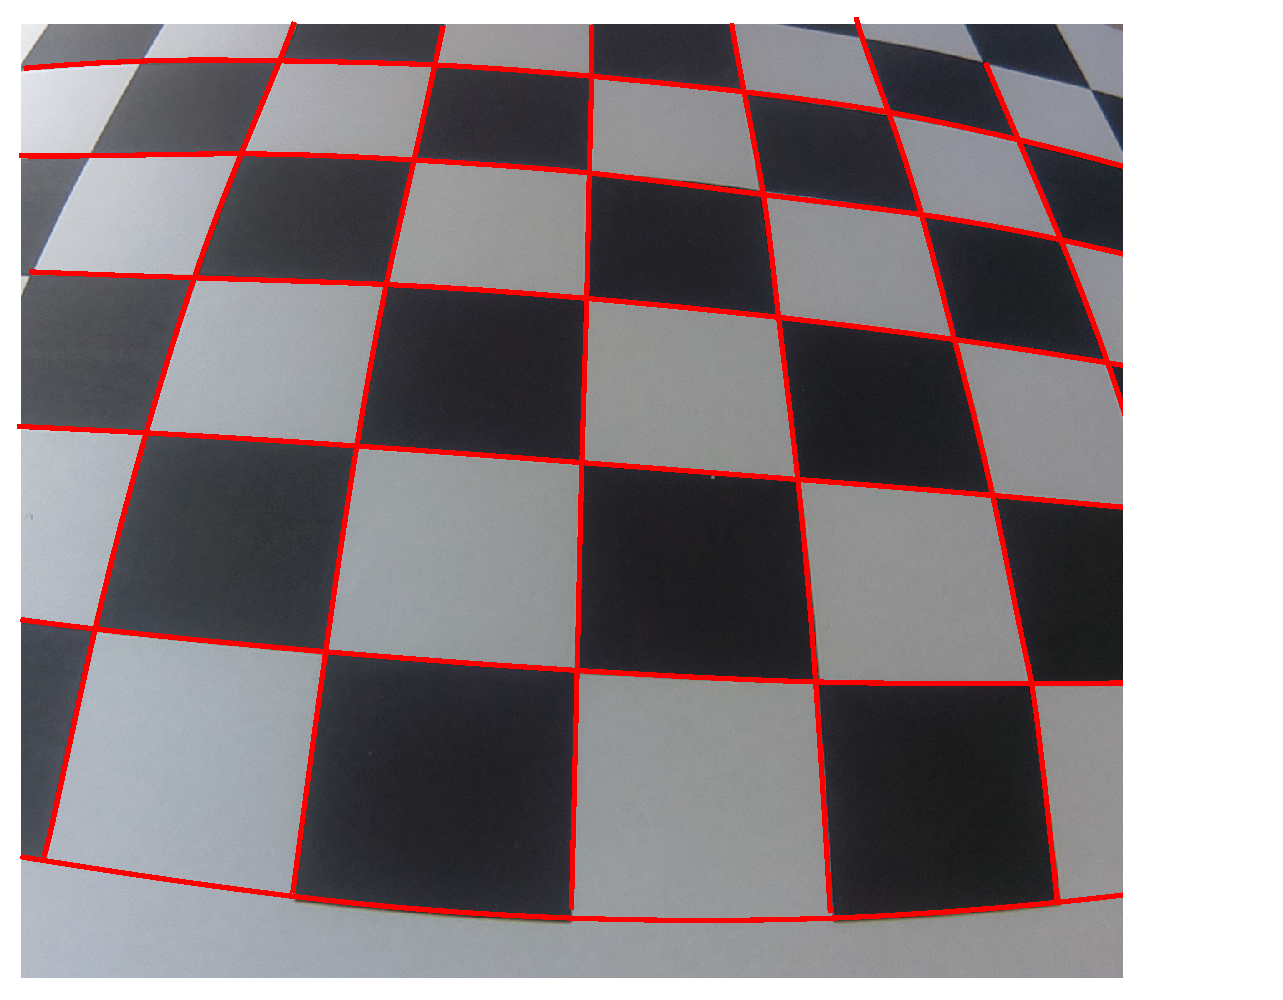
\includegraphics[scale=.35]{images/calibrationRaspi.eps}
	\caption{vor Kalibrierung}
	\label{fig:calibDist}
\end{subfigure}%
\begin{subfigure}{.5\textwidth}
	\centering
	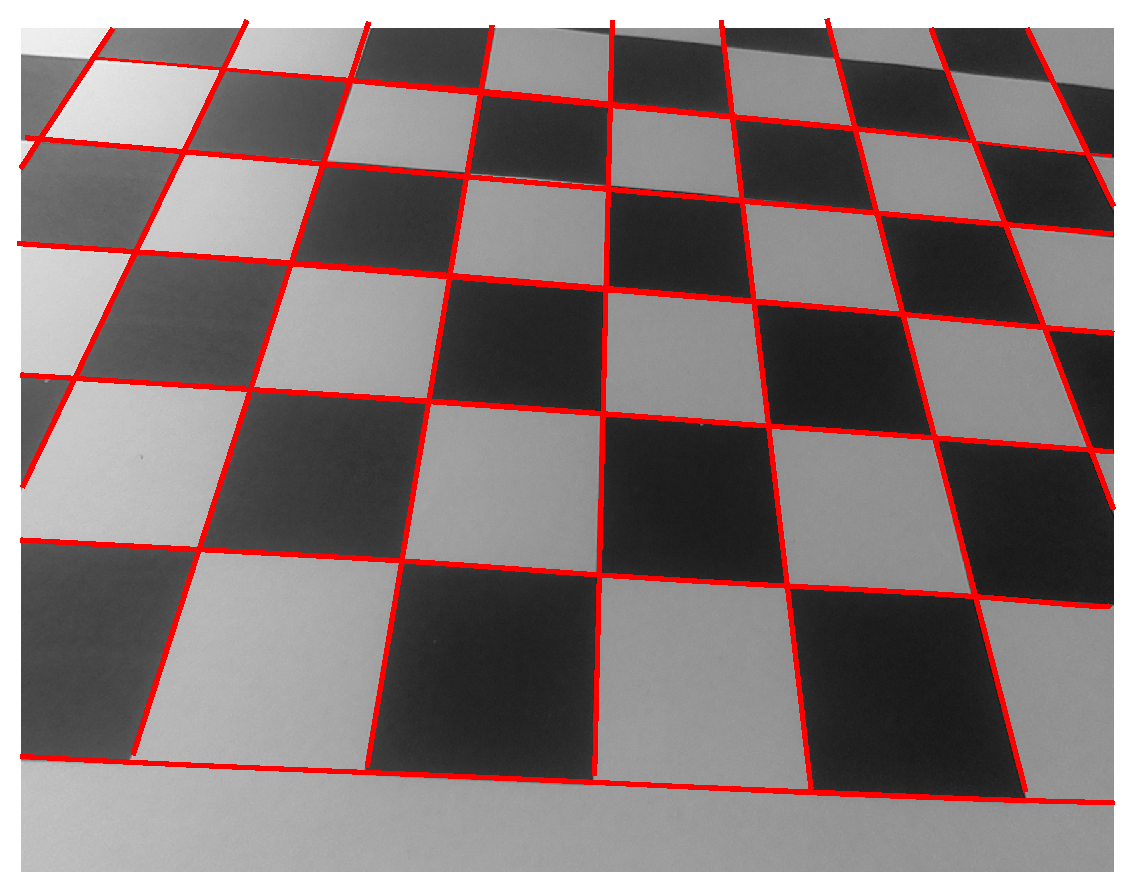
\includegraphics[scale=.4]{images/calibrationRaspi2.eps}
	\caption{nach Kalibrierung und Entzerrung}
	\label{fig:calibUndist}
\end{subfigure}
\caption{Kamerakalibrierung}
\label{fig:calib}
\end{figure}


\section{Detektion der Samples} \todo{Umbennenen}

Nach der Kamerakalibrierung und entsprechender Entzerrung werden die Bildkoordinaten der Samples bestimmt. Dazu ist wird ein Blob-Detektor \ref{s:blob} benutzt. Um die Samples korrekt von den Kreislinien, sowie den Liniensegmenten trennen zu können, ist es wichtig dass die Umgebung eines Samples frei ist. \todo{Formulierung}.

Filtert Farbe (schwarz), kleine Flächen werden verworfen, Kreisförmigkeit, Konvexität

\section{Ellipsen-Detektion}
\label{s:ellipseDetection}
Nachdem die Sample-Positionen bestimmt wurden, muss für jeden Sample entschieden werden, auf welcher der Kreislinien er liegt. Da die Kreise, bedingt durch perspektivische Verzerrung, zu  Ellipsen werden, wird eine Verfahren 
benötigt, dass Ellipsen erkennt. 

Zunächst werden die Kanten mit Hilfe von Canny (\ref{s:canny}) detektiert (siehe Abbildung \ref{fig:canny}). 

\begin{figure}[!htb]
	\centering
	\begin{subfigure}{.5\textwidth}
		\centering
		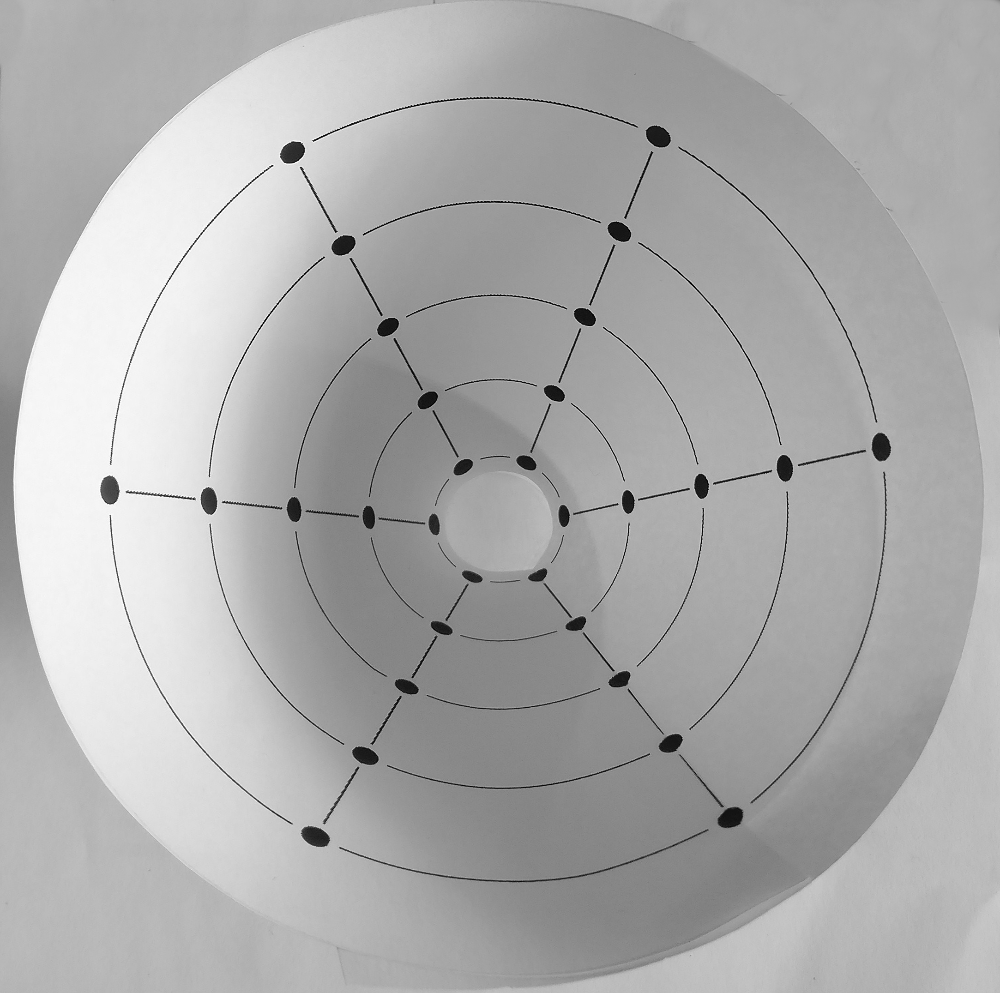
\includegraphics[width=.9\textwidth]{images/grey.png}
		\caption{Grauwertbild}
		\label{fig:beforeCanny}
	\end{subfigure}%
	\begin{subfigure}{.5\textwidth}
		\centering
		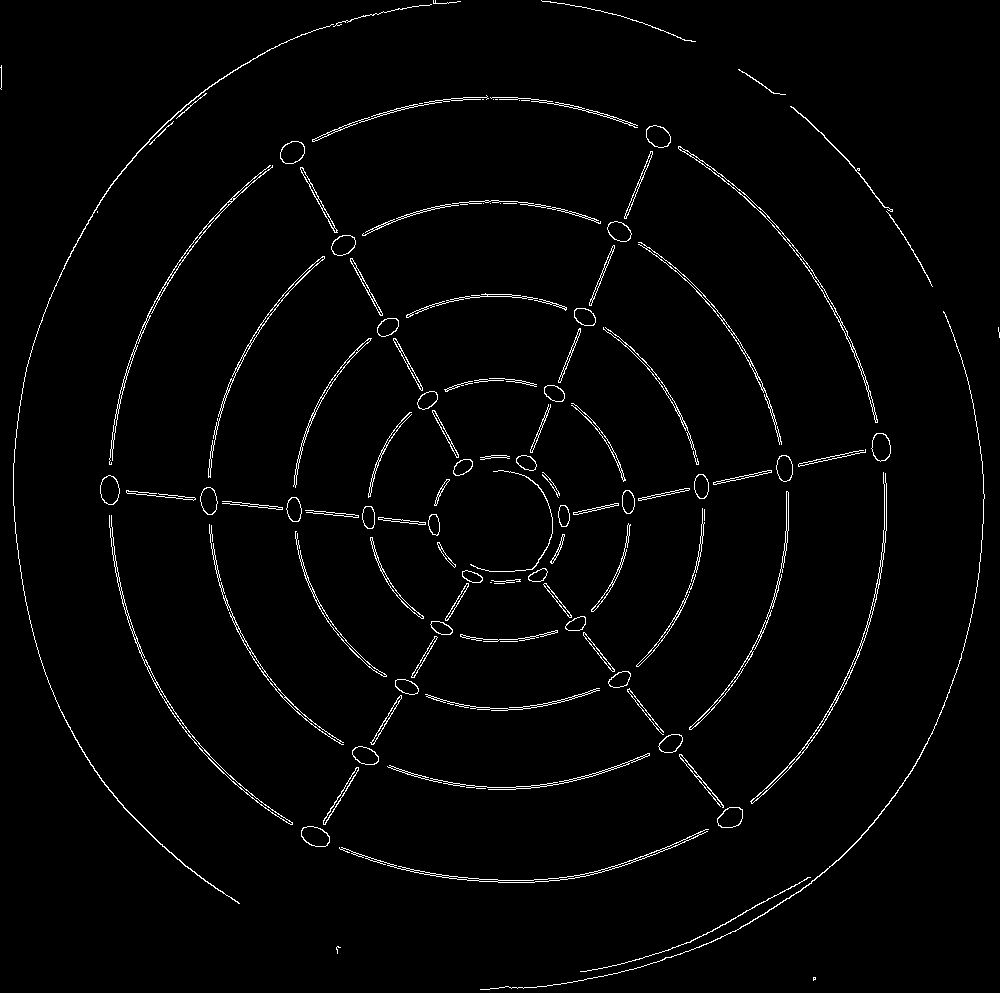
\includegraphics[width=.9\textwidth]{images/canny.png}
		\caption{Canny-Kanten}
		\label{fig:afterCanny}
	\end{subfigure}
	\caption{Canny-Kantendetektion auf Grauwertbild}
	\label{fig:canny}
\end{figure}

Anschließend versuchen wir möglichst genau das Zentrum der innersten Ellipsen zu bestimmen.
Wir benutzen dafür Hough-Transformationen, um Linien im Canny-Bild zu \todo{hier passendes Wort einfügen}.
Es werden anschließend Schnittpunkte aller Liniensegmente bestimmt. Bedingt durch Ungenauigkeiten beim Ausschneiden und Zusammenlegen im Kegel, schneiden sich nicht alle Liniensegmente in einem Punkt.
Darüber hinaus werden, auf Grund der Liniendicke auf dem Kalibrierungsmuster, durch Canny viele Linien doppelt erkannt. Auch ein inhomogener Hintergrund, erschwert die Schnittpunktsbestimmung. Um also möglichst robust einen Kandidaten auszuwählen, wird zuerst der Median der $x$-Koordinaten der Schnittpunkte und dann der Median der $y$-Koordinaten bestimmt. Die erhaltenen Koordinaten bilden den Schnittpunkt (siehe Abbildung \ref{fig:houghLines}).

\begin{figure}[!htb]
	\centering
	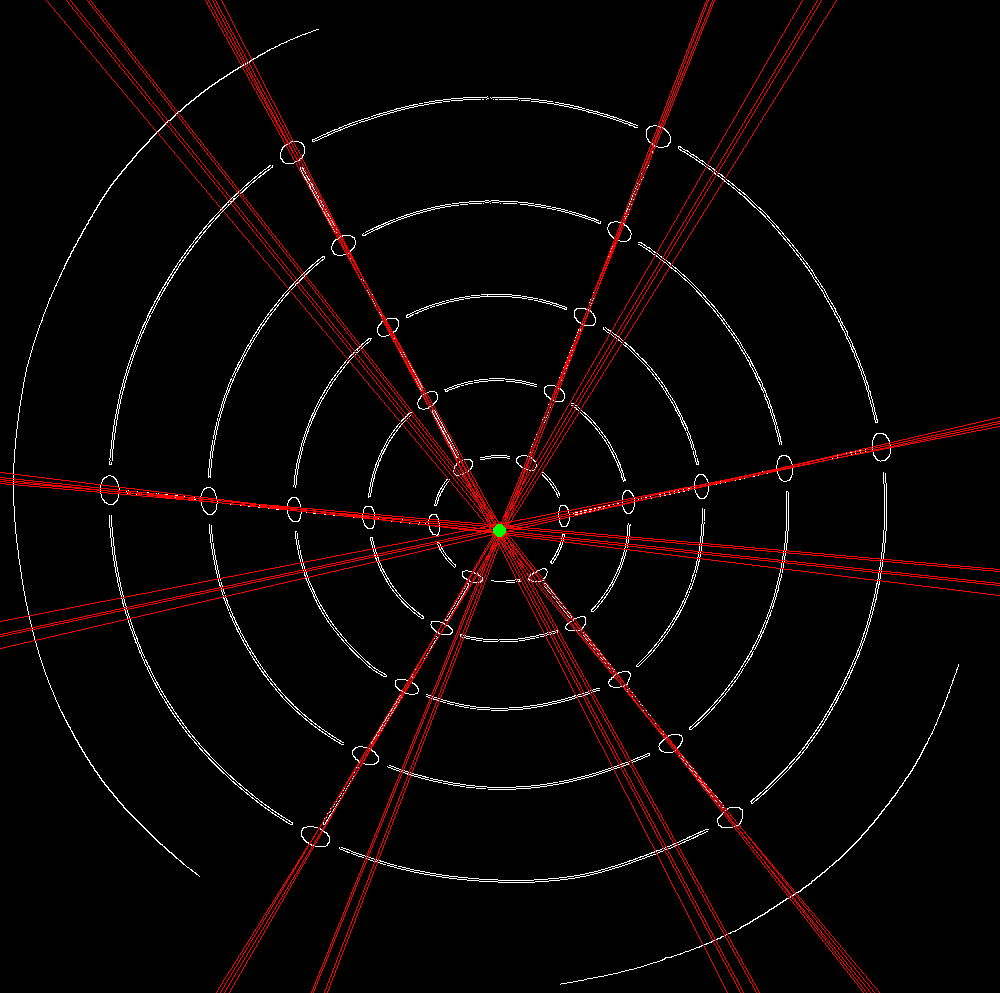
\includegraphics[scale=.25]{images/houghLines.png}
	\caption{Hough-Transformation zur Linien-Detektion (in rot gekennzeichnet) und bestimmter Schnittpunkt (in grün) }
	\label{fig:houghLines}
\end{figure}

Von diesem Schnittpunkt aus werden, in einer vorher definierte Anzahl, gleichmäßig, in alle Richtungen Strahlen ausgesendet. \todo{Komma-Setzung}. 
Trifft ein Strahl ein weißes Pixel, wird dessen Position gekennzeichnet, trifft er den Rand des Bildes, wird er ignoriert. In Abbildung \ref{fig:rayCastWOE} sind die getroffenen weißen Pixel und der zugehörige Aussendepunkt eingezeichnet. 

\begin{figure}[!htb]
	\centering
	\begin{subfigure}{.5\textwidth}
		\centering
		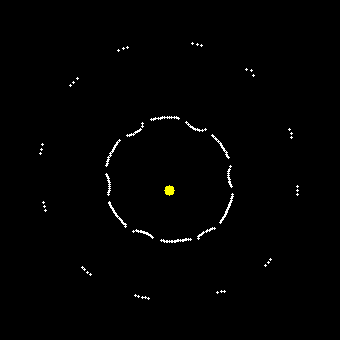
\includegraphics[width=.9\textwidth]{images/rayCast0.png}
		\caption{bestimme Pixel-Positionen}
		\label{fig:rayCastWOE}
	\end{subfigure}%
	\begin{subfigure}{.5\textwidth}
		\centering
		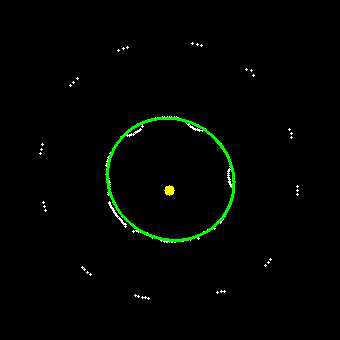
\includegraphics[width=.9\textwidth]{images/rayCast0Ellipse.png}
		\caption{bestimme Ellipse (grün)}
		\label{fig:rayCastWE}
	\end{subfigure}
	\caption{Ellipsendetektion: bestimme Pixel-Positionen (weiß), Aussendepunkt (gelb)}
	\label{fig:rayCast}
\end{figure}

Mit Hilfe der Postionen der weißen Pixel, wird anschließend durch RANSAC (siehe Kapitel \ref{s:ransac}) eine Ellipse geschätzt. Um die, für RANSAC benötigte, Distanz zu berechnen, wird das Verfahren aus Kapitel \ref{sc:distPointEllipse} genutzt, was die exakte euklidische Distanz eines Punktes zu einer Ellipse bestimmt. Ein Verfahren wie das Verfahren der kleinsten Quadraten funktioniert hier nicht, dass die weißen Pixel bezüglich einer zu bestimmen Ellipse, Ausreißer behaftet sind. Wird zum Beispiel auf Grund schlechter Lichtverhältnisse eine Kreislinie nicht deutlich aufgenommen, kann es in dem Kantenbild (Abbildung \ref{fig:canny}) zu "`Löchern"' in den Kreislinien und folglich treffen die ausgesendeten Strahlen die nächst äußere Kreislinie (siehe Abbildung \ref{fig:rayCastR}). Da die Laufzeit nicht im Vordergrund steht, kann eine großzügige Schätzung des Fehleranteils von $\epsilon = 0.4$ mit einer gewünschten Wahrscheinlichkeit $p = 0.9999$ gewählt werden, was zu einer Mindestanzahl an Iterationen von circa $200$ führt (siehe Kapitel \ref{s:ransac}). Die letztendlich bestimmen Ellipsen sind beispielhaft in Abbildung \ref{fig:detectedEllipses} zu sehen.  


\begin{figure}[!htb]
	\centering
	\begin{subfigure}{.5\textwidth}
		\centering
		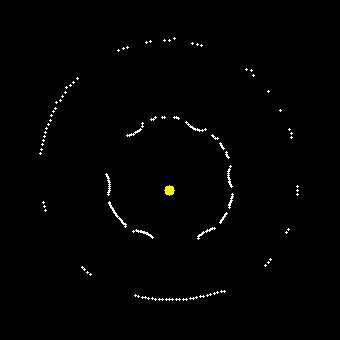
\includegraphics[scale=.6]{images/rayCastRobust.png}
		\caption{bestimme Pixel-Positionen}
		\label{fig:rayCastRWOE}
	\end{subfigure}%
	\begin{subfigure}{.5\textwidth}
		\centering
		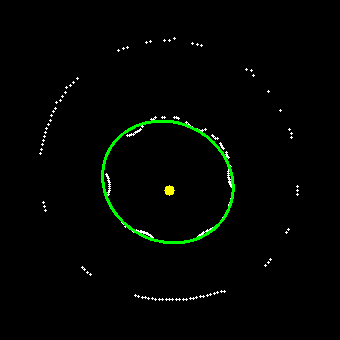
\includegraphics[scale=.6]{images/rayCastRobustEllipse.png}
		\caption{bestimme Ellipse (grün)}
		\label{fig:rayCastRWE}
	\end{subfigure}
	\caption{Ellipsendetektion bei Ausreißern}
	\label{fig:rayCastR}
\end{figure}


\begin{figure}[!htb]
	\centering
	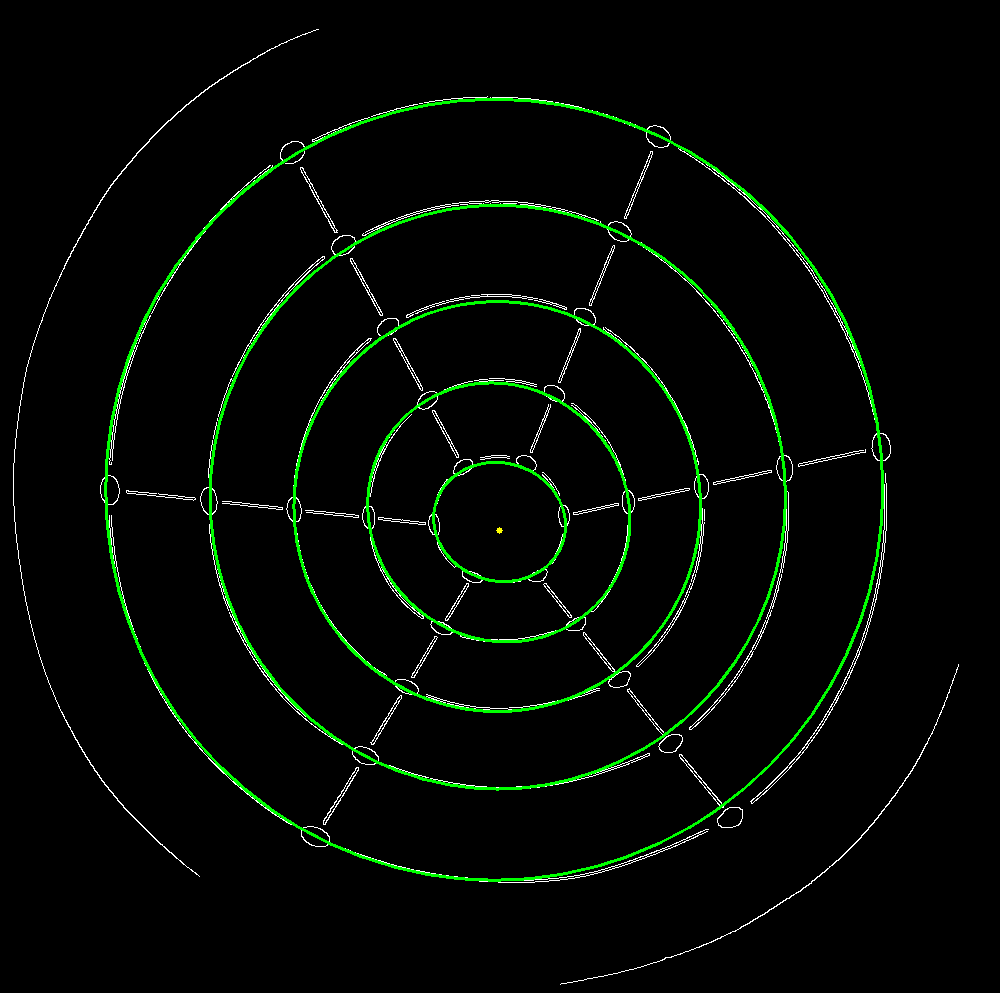
\includegraphics[scale=.25]{images/detectedEllipses.png}
	\caption{Ellipsen}
	\label{fig:detectedEllipses}
\end{figure}

\newpage
\section{Zuordnung der Punkte}
\label{s:pointMapping}
Nach der Bestimmung der Ellipsen muss jede Sample-Positionen der zugehörigen Kreislinie, sowie Liniensegment zugeordnet werden, um seine Position auf dem Kegel bestimmen zu können. 
Zunächst wird für jeden Punkte diejenige Kreislinie ausgewählt, dessen zugehörige Ellipse die kürzeste Distanz zu ihm hat (siehe Abbildung \ref{fig:ellipseMapping}).

Mit Hilfe dieser Zuordnung können die Ellipsen aus Kapitel \ref{s:ellipseDetection} erneut geschätzt werden. Diesmal wird das Verfahren der kleinsten Quadrate genutzt, da nur die ausreißerfreihen Samples als Messdaten dienen und wir eine optimale Lösung für alle Samples anstreben.  

Um nun die Samples auch ihren Liniensegmenten zuzuordnen, wird zunächst der Mittelpunkt der Samples auf der innersten Ellipse bestimmt. Anschließend werden die Samples auf der innersten Ellipsen nach dem Winkel der Verbindungslinien zwischen Sample und Mittelpunkt mit der $X$-Achse sortiert. 
Die restlichen Samples können nicht nach dem gleichen Schema sortiert werden, da der bestimme Mittelpunkt nicht der genaue Schnittpunkt aller Liniensegmente ist. Der Winkel zwischen der Samples auf einem Liniensegment und des bestimmen Mittelpunkts ist also nicht identisch. 
Stattdessen wird für jedes Sample  auf den darauffolgenden Ellipsen, das Sample auf der vorherigen Ellipse mit der kürzesten Distanz bestimmt. 

Die Samples können nun entsprechend sortiert werden. Die zugeordneten Liniensegmente sind exemplarisch in Abbildung \ref{fig:lineMapping} zu sehen. 


\begin{figure}[!htb]
	\centering
	\begin{subfigure}{.5\textwidth}
		\centering
		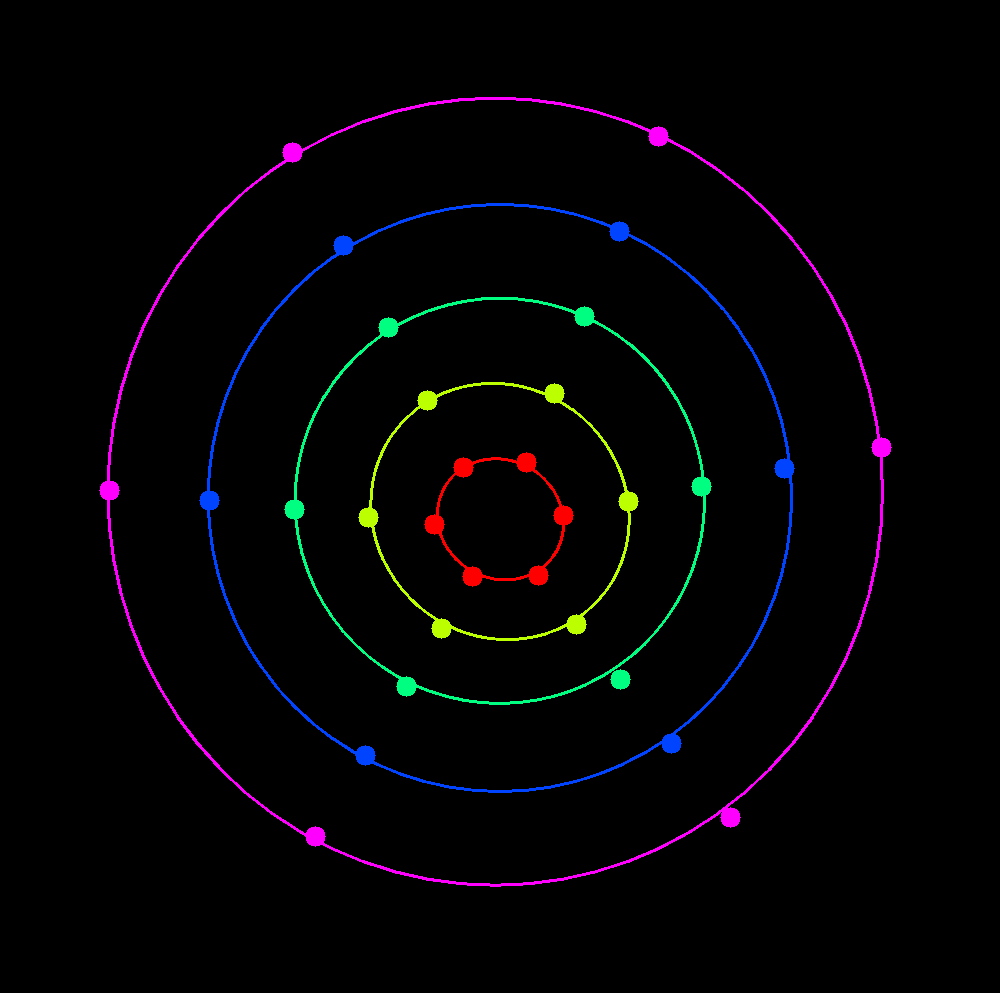
\includegraphics[width=.9\textwidth]{images/ellipseMapping.png}
		\caption{Zuordnung von Punkten zu Ellipsen}
		\label{fig:ellipseMapping}
	\end{subfigure}%
	\begin{subfigure}{.5\textwidth}
		\centering
		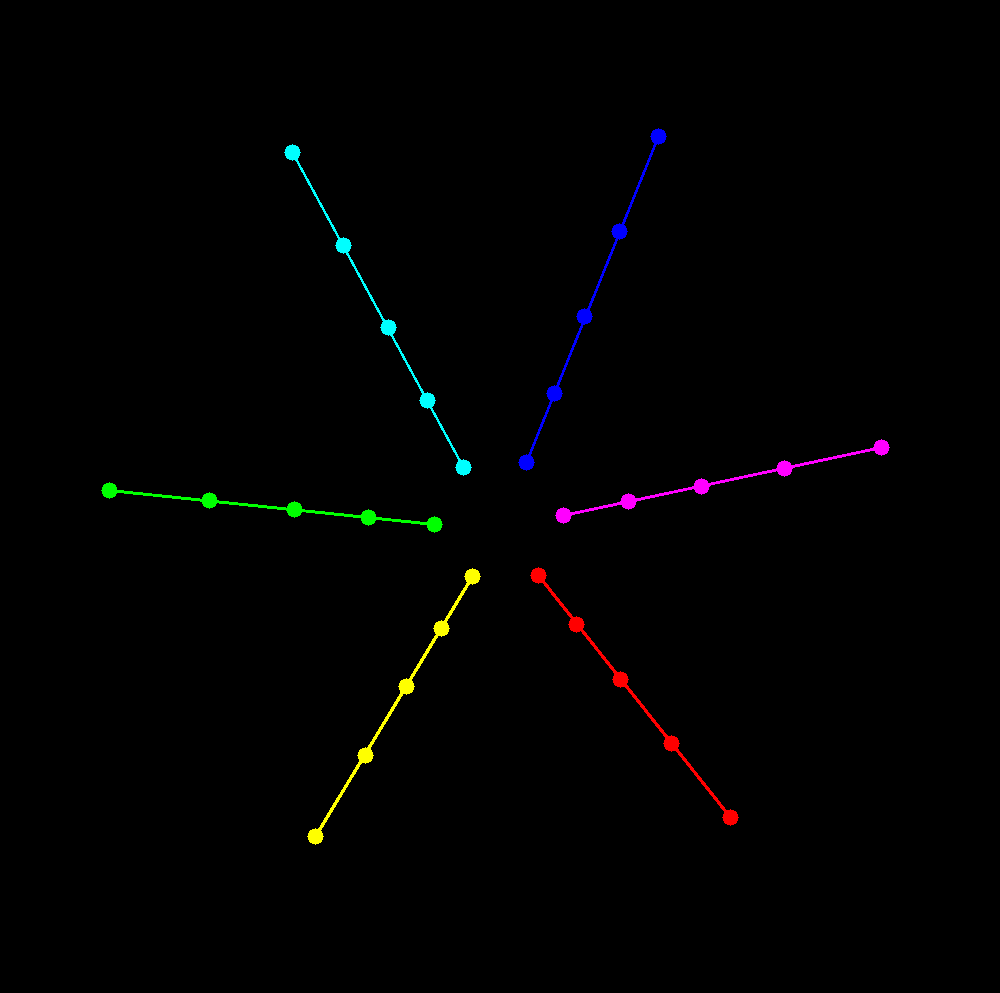
\includegraphics[width=.9\textwidth]{images/lineMapping.png}
		\caption{Zuordnung von Punkten zu Liniensegmenten}
		\label{fig:lineMapping}
	\end{subfigure}
	\caption{Zuordnung von Punkten zu Ellipsen (links) und Liniensegmenten (rechts)}
	\label{fig:rayCastR}
\end{figure}


\section{Weltkoordinaten bestimmen}

Aus dem vorherigen Kapitel wissen wir nun für jedes Sample den Ort auf dem Kegel. Wir können die 3D-Koordinaten also folgendermaßen angeben:

Ohne Beschränkung der Allgemeinheit, seien die Ellipsen $i = 0,\dotsc,n - 1$ aufsteigend nach ihrer "`Größe"'\footnote{Etwas formaler, könnte man die Ellipsen hier nach ihrem Flächeninhalt sortieren. Für Ellipsen $E_0(x_0,y_0,a_0, b_0, \theta_0)$ und $E_1(x_1,y_1,a_1, b_1,\theta_1)$ gilt $E_0 \leq E_1$ g.d.w. $\pi\cdot a_0 \cdot b_0 \leq \pi \cdot a_1 \cdot b_1$} sortiert, so wie es das Verfahren in \ref{s:ellipseDetection} beschreibt.
Außerdem seien die Liniensegmente $j = 0,\dotsc,m - 1$ aufsteigend nach Winkel mit der $X$-Achse, wie in \ref{s:pointMapping} beschrieben, sortiert. 
Eine Sample kann also eindeutig durch ein Tupel $(i,j) \in [0,n-1]\times [0,m-1]$ identifiziert werden und $(x_{ij},y_{ij},z_{ij})$ bezeichne seine Koordinaten im Weltkoordinatensystem. 

Analog zur parametrischen Darstellung von Kegelstümpfen (Gleichung \ref{eq:paramFrustum}) in Kapitel \ref{s:cone} ergibt sich:

\begin{equation*}
\begin{aligned}
x_{ij} &= r_i~cos \theta_j \\
y_{ij} &= h_i\\
z_{ij} &= r_i~sin \theta_j
\end{aligned}
\end{equation*}
$\forall (i,j) \in [0,n-1]\times [0,m-1]$ mit 
\begin{equation*}
\begin{aligned}
r_i &= r + \frac{i}{n}\cdot(R - r) \quad&\forall i\in[0,n-1]\\
h_i &= \frac{i}{n}\cdot\Delta H &\forall i\in[0,n-1]\\
\theta_j &= \frac{j}{m-1} \cdot  2\pi  &\forall j\in[0,m-1]
\end{aligned}
\end{equation*}

\section{Entfaltung}
Die eigentliche Entfaltung des Kegels, mit zwei unterschiedlichen Ansätzen realisiert werden. 
Die erste Möglichkeit ist die \textit{Vorwärtsentfaltung}. Hierbei wird für jedes Pixel auf dem Kegelbild eine 3D-Koordinate durch geeignete Interpolation bestimmt und dann auf die Mantelfläche abgebildet. Beim zweiten Ansatz der  \textit{Rückwärtsentfaltung} wird ein Punkt von der Mantelfläche zurück auf den Kegel abgebildet und von dort mit einer Projektionsmatrix auf die Bildebene projiziert und dann interpoliert. 

Im folgenden wird genauer auf beide Verfahren eingegangen, sowie deren Probleme erläutert. \todo{hier schon erläutern oder erst in späteren kapiteln?}

\subsection{Vorwärtsentfaltung}
Bei der \textit{Vorwärtsentfaltung} muss wie oben erwähnt zu jedem Pixel die zugehörige 3D Koordinate im Weltkoordinatensystem berechnet werden. Da bisher jedoch nur die Postionen der Samples bekannt sind muss hier 

Zunächst betrachten wir diejenigen Pixel, die sich weder auf einer Kreislinie, noch auf einem Liniensegment befinden. Es gibt zu einem Pixel $P$ also immer vier Sample-Nachbarn $(bl, br, tr, tl)$. Diese Situation ist in Abbildung \ref{fig:radialInterpolation} illustriert. 

Nachdem die vier Nachbarn bestimmt wurden, können im ersten Schritt die Abstande $d_1$ und $d_2$ zu inneren Ellipse $E_b$, respektive äußeren Ellipse $E_t$ berechnet werden. Mithilfe dieser Abständen kann nun eine \textit{Interpolationsellipse}~$E_1$ definiert werden als:
\begin{equation*}
	E_{int} = \left(\frac{d_1}{d_1 + d_2}\right) \cdot E_t + \left(\frac{d_2}{d_1 + d_2}\right) E_b
\end{equation*}

Wo eine Multiplikation mit einem Skalar alle Charakteristika einer Ellipse skaliert\footnote{der Drehwinkel $\theta$ wird hierbei anschließend$\mod 2\pi$ gerechnet}, und eine Addition elementweise addiert. Im nächsten Schritt wird der Schnittpunkt $L$ mit dem Liniensegment $\overline{bltl}$, sowie der Schnittpunkt $R$ mit dem Liniensegment $\overline{brtr}$ bestimmt. 

Da sich $tl$, $L$ und $bl$ nun auf einem gemeinsamen Liniensegment befinden, kann bezüglich der Weltkoordinaten linear interpoliert werden. Analoges gilt für $R$. 

Die drei Punkte $(L,P, R)$ befinden sich auf der Interpolationsellipse und somit können die  Winkel $(\phi_L, \phi_P, \phi_R)$ bezüglich des Ellipsenkoordinatensystems bestimmt werden. 


Die auf Liniensegmenten befindlichen Punkte werden dabei einfach linear interpoliert. Die Pixel, die sich auf Kreislinien befinden werden über Winkel interpoliert. 

\begin{figure}[!htb]
	\centering
	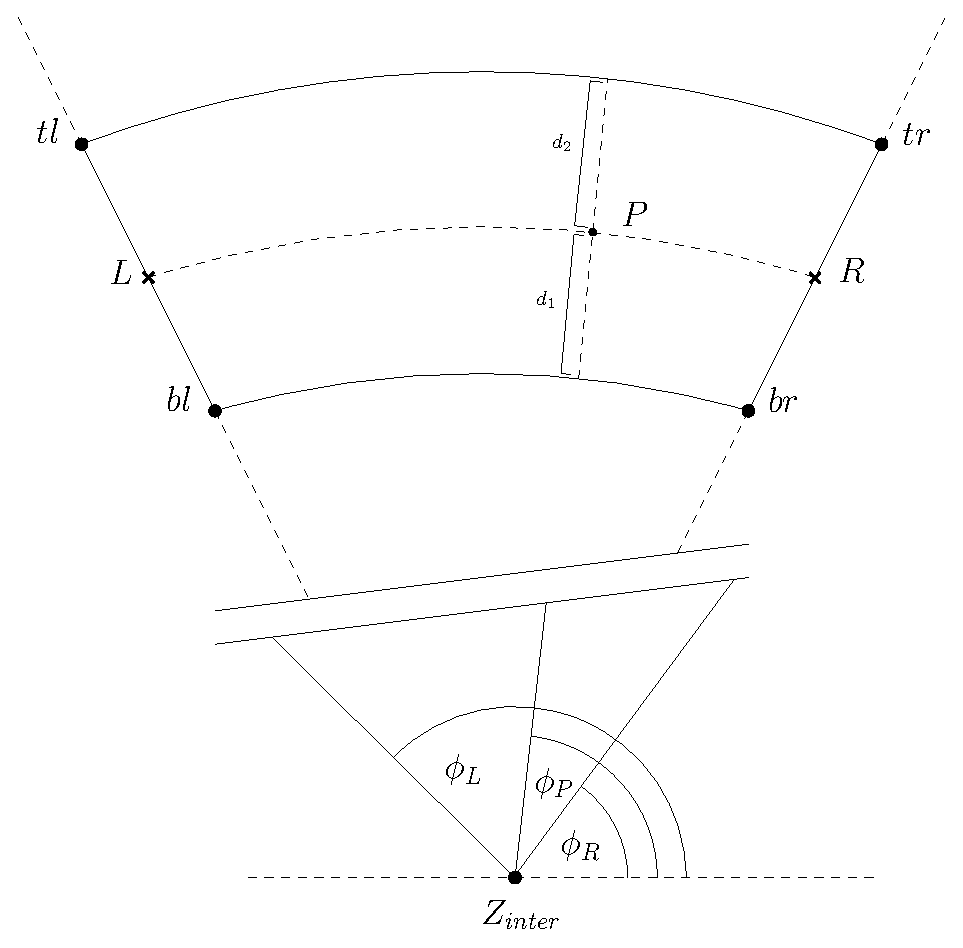
\includegraphics[scale=.6]{images/radialInterpolation.eps}
	\caption{Interpolation}
	\label{fig:radialInterpolation}
\end{figure}



Probleme: bei der skizze geht ein punkt auf der kreislinie $E_t$ mit der y-koordinate niemals über die y koordinate von tl und tr hinaus.

bei der transfomrtaiton entstehen unvermeidbare löcher.







\subsection{Rückwärtsentfaltung}
Projektionsmatrix bestimmen
